\chapter{平面向量及其应用}

本章介绍平面上的向量。有两个难点,第一,平面向量是第一次碰到,难以快速熟悉并掌握,需要花大力气,其次,向量是连接代数和几何的桥梁,容易出大题,计算量可大可小。所以平面向量的学习需要反复研读定义,深刻理解定义提出的背景,还须结合几何,多画图,借助图形展开思考。

本章要点:
\begin{itemize}
    \item 平面向量及其几何意义。
    \item 余弦定理和正弦定理。
\end{itemize}

\newpage
\section{平面向量的概念}

都是定义,没啥难点。向量就是带方向的量。

可以这么理解,如果描述一维空间的坐标,则使用标量即可,没有方向,或者只有两个方向,前后,用实数的正负即可。如果描述二维空间的坐标,则必须使用两个标量,组合在一起就是向量。

教材中说道向量的三元素:起点、方向、长度。其实只有方向和长度,我们不太关心起点,起点是可以移动的。从后续的平行和相等的定义也可以看出,起点并没有要求。

这里容易忽略一个关键点,即模和方向是向量的固有属性。所谓的固定属性就是它们不随参考系的变化而变化,这点在学习到第3节的时候需要特别注意!XML。






\newpage
\section{平面向量的运算}

本节要点:
\begin{itemize}
    \item 掌握向量的运算的概念;
    \item 掌握向量的运算法则;
    \item 理解向量运算的几何意义。
\end{itemize}

\begin{tcolorbox}
本节将向量作为一个整体,或者说将向量作为一个一类数,定义了运算法则。下一节将向量和实数关联讨论运算法则,注意这两节的区别。
\end{tcolorbox}

本节对向量的运算做了定义,特别是内积,“6.2.4向量的数量积”定义了内积,这个概念是实数没有的,需要熟悉,把该小节的所有例题全部吃透!反复吃透!

加法的交换律和结合律:
\begin{align*}
&\boldsymbol{a}+\boldsymbol{b}=\boldsymbol{b}+\boldsymbol{a} \\
&\left( \boldsymbol{a}+\boldsymbol{b} \right) +\boldsymbol{c}=\boldsymbol{a}+\left( \boldsymbol{b}+\boldsymbol{c} \right)
\end{align*}

数乘的结合律和分配律:
\begin{align*}
&\lambda \left( \mu \boldsymbol{a} \right) =\left( \lambda \mu \right) \boldsymbol{a} \\
&\left( \lambda +\mu \right) \boldsymbol{a}=\lambda \boldsymbol{a}+\mu \boldsymbol{a} \\
&\lambda \left( \boldsymbol{a}+\boldsymbol{b} \right) =\lambda \boldsymbol{a}+\lambda \boldsymbol{b}
\end{align*}

内积的交换律和分配律,特别注意,内积没有结合律:
\begin{align*}
&\boldsymbol{a}\cdot \boldsymbol{b}=\boldsymbol{b}\cdot \boldsymbol{a} \\
&\boldsymbol{a}\cdot \left( \boldsymbol{b}+\boldsymbol{c} \right) =\boldsymbol{a}\cdot \boldsymbol{b}+\boldsymbol{a}\cdot \boldsymbol{c}
\end{align*}

两个重要的不等式:
\begin{itemize}
    \item $\left| \boldsymbol{a}+\boldsymbol{b} \right|\leqslant \left| \boldsymbol{a} \right|+\left| \boldsymbol{b} \right|$,当且仅当$\boldsymbol{a},\boldsymbol{c}$同向时等号成立;
    \item $\left| \boldsymbol{a}\cdot \boldsymbol{b} \right|\leqslant \left| \boldsymbol{a} \right|\cdot \left| \boldsymbol{b} \right|$,当且仅当$\boldsymbol{a},\boldsymbol{c}$平行时等号成立。
\end{itemize}

两个与几何相关的判断,也即数乘和内积的几何意义:
\begin{itemize}
    \item $\boldsymbol{a}=\lambda \boldsymbol{b},\lambda \ne 0\Leftrightarrow \boldsymbol{a},\boldsymbol{b}\text{平行}$;
    \item $\boldsymbol{a}\cdot \boldsymbol{b}=0\Leftrightarrow \boldsymbol{a},\boldsymbol{b}\text{垂直}$。
\end{itemize}

\begin{tcolorbox}
向量是联系代数和几何的有力工具,所以必须深刻理解向量及其运算的几何意义。向量描述了几何的点,向量的集合便是点的集合,可以构成直线、圆、弧、曲线等等。向量的运算描述了这些点和线的关系。
\end{tcolorbox}

\begin{tcolorbox}
教材从力的做功定义向量内积,略有唐突,但考虑到高中阶段背景知识也只能如此。其实向量的相乘还有一个外积,两个积合起来还有更深刻的物理意义,XML。
\end{tcolorbox}

~

\begin{example}[复习巩固7]
已知$\boldsymbol{a},\boldsymbol{b}$为两个非零向量,
\begin{enumerate}
    \item 求作向量$\boldsymbol{a}+\boldsymbol{b},\boldsymbol{a}-\boldsymbol{b}$;
    \item 当向量$\boldsymbol{a},\boldsymbol{b}$成什么位置关系时,满足$\left| \boldsymbol{a}+\boldsymbol{b} \right|=\left| \boldsymbol{a}-\boldsymbol{b} \right|$?(不要求证明)。
\end{enumerate}
\end{example}

解:

只讨论(2),直觉发现要求$\boldsymbol{a}\bot \boldsymbol{b}$。由于涉及向量的坐标表示,所以这里不要求证明,但我们在学习完6.3后回头再证明该题。
令$\boldsymbol{a}=\left( x_{\boldsymbol{a}},y_{\boldsymbol{a}} \right) ,\boldsymbol{b}=\left( x_{\boldsymbol{b}},y_{\boldsymbol{b}} \right) $,可得:
\begin{align*}
&\because \left| \boldsymbol{a}+\boldsymbol{b} \right|=\left| \boldsymbol{a}-\boldsymbol{b} \right| \\
&\therefore \left( x_{\boldsymbol{a}}+x_{\boldsymbol{b}} \right) ^2+\left( y_{\boldsymbol{a}}+y_{\boldsymbol{b}} \right) ^2=\left( x_{\boldsymbol{a}}-x_{\boldsymbol{b}} \right) ^2+\left( y_{\boldsymbol{a}}-y_{\boldsymbol{b}} \right) ^2 \\
&\therefore 2x_{\boldsymbol{a}}x_{\boldsymbol{b}}+2y_{\boldsymbol{a}}y_{\boldsymbol{b}}=-2x_{\boldsymbol{a}}x_{\boldsymbol{b}}-2y_{\boldsymbol{a}}y_{\boldsymbol{b}} \\
&\therefore x_{\boldsymbol{a}}x_{\boldsymbol{b}}+y_{\boldsymbol{a}}y_{\boldsymbol{b}}=0 \\
&\therefore \boldsymbol{a}\cdot \boldsymbol{b}=0
\end{align*}

~

\begin{example}[复习巩固12,难度:$\star $]
求证:
\[
\left( \lambda \boldsymbol{a} \right) \cdot \boldsymbol{b}=\lambda \left( \boldsymbol{a}\cdot \boldsymbol{b} \right) =\boldsymbol{a}\cdot \left( \lambda \boldsymbol{b} \right)
\]
\end{example}

解:

只证明第一个等号:
\begin{align*}
&\left( \lambda \boldsymbol{a} \right) \cdot \boldsymbol{b}=\left| \lambda \boldsymbol{a} \right|\cdot \left| \boldsymbol{b} \right|\cdot \cos \alpha =\left| \lambda \right|\cdot \left| \boldsymbol{a} \right|\cdot \left| \boldsymbol{b} \right|\cdot \cos \alpha \\
&\lambda \left( \boldsymbol{a}\cdot \boldsymbol{b} \right) =\lambda \left( \left| \boldsymbol{a} \right|\cdot \left| \boldsymbol{b} \right|\cdot \cos \alpha \right)
\end{align*}
再从$\lambda <0,>0,=0$三个方面讨论即可,略。

\begin{tcolorbox}
该关系式是内积的性质,证明性质,都从定义入手。
\end{tcolorbox}

~

\begin{example}[拓广探索23,难度:$\star $]
已知$O$为平行四边形$ABCD$所在平面内一点,且向量$\overrightarrow{OA},\overrightarrow{OC},\overrightarrow{OB},\overrightarrow{OD}$满足等式$\overrightarrow{OA}+\overrightarrow{OC}=\overrightarrow{OB}+\overrightarrow{OD}$。
\begin{enumerate}
    \item 做出满足条件的四边形$ABCD$。
    \item 四边形$ABCD$有什么特点?请证明你的猜想。
\end{enumerate}
\end{example}

\begin{figure}[h]
\centering
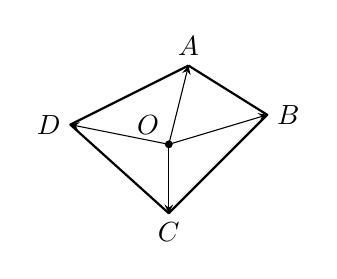
\begin{tikzpicture}[line join=round, scale=1.25]
\pgfmathparse{0.6/1.5}
\coordinate[label=above left:{$O$}] (O) at (0,0);
\coordinate[label=left:{$D$}] (D) at (-1,0.2);
\coordinate[label=right:{$B$}] (B) at (1,0.3);
\coordinate[label=below:{$C$}] (C) at (0,-0.7);
\coordinate[label=above:{$A$}] (A) at (0.2,0.8);
\fill (O) circle (\pgfmathresult mm);
\draw[thick] (A)--(B)--(C)--(D)--(A);
\draw[-stealth] (O)--(A);
\draw[-stealth] (O)--(B);
\draw[-stealth] (O)--(C);
\draw[-stealth] (O)--(D);
\end{tikzpicture}
\end{figure}

解:

$\overrightarrow{OA}+\overrightarrow{OC}$表示两向量和,但几何上起点相同,所以很难由此判断出四边形的特点,最好是首尾相连,且去掉$O$。
将等式变换化简:
\begin{align*}
&\overrightarrow{OA}+\overrightarrow{OC}=\overrightarrow{OB}+\overrightarrow{OD} \\
&\overrightarrow{OA}-\overrightarrow{OB}=\overrightarrow{OD}-\overrightarrow{OC} \\
&\overrightarrow{BO}+\overrightarrow{OA}=\overrightarrow{CO}+\overrightarrow{OD} \\
&\overrightarrow{BA}=\overrightarrow{CD}
\end{align*}
对边相等且平行,易得为平行四边形。

\begin{tcolorbox}
此题考察向量运算的几何意义,粗看较为抽象,但依然有思路可循。
\end{tcolorbox}

~

\begin{example}[拓广探索24,难度:$\star $]
如图,在$\odot C$中,是不是只需知道$\odot C$的半径或弦$AB$的长度,就可以求出$\overrightarrow{AB}\cdot \overrightarrow{AC}$的值?
\end{example}

\begin{figure}[h]
\centering
\begin{tikzpicture}[line join=round, scale=1.25]
\pgfmathparse{0.6/1.2}
\draw[thick] (0,0) circle(1);
\coordinate[label=above:{$C$}] (C) at (0,0);
\coordinate[label=left: {$A$}] (A) at (-0.72,-0.7);
\coordinate[label=right:{$B$}] (B) at (0.88,-0.47);
\fill (C) circle (\pgfmathresult mm);
\draw[-stealth] (A)--(C);
\draw[-stealth] (A)--(B);
\pic["$\alpha $",draw,angle radius=0.5cm,angle eccentricity=1.5] {angle=B--A--C};
\end{tikzpicture}
\end{figure}

解:

\begin{align*}
&\because \overrightarrow{AB}\cdot \overrightarrow{AC}=\left| \overrightarrow{AB} \right|\cdot \left| \overrightarrow{AC} \right|\cdot \cos \alpha \\
&\because \cos \alpha =\frac{\left| \overrightarrow{AC} \right|^2+\left| \overrightarrow{AB} \right|^2-\left| \overrightarrow{CB} \right|^2}{2\cdot \left| \overrightarrow{AC} \right|\cdot \left| \overrightarrow{AB} \right|} \\
&\because \left| \overrightarrow{AC} \right|=\left| \overrightarrow{CB} \right| \\
&\therefore \overrightarrow{AB}\cdot \overrightarrow{AC}=\frac{\left| \overrightarrow{AB} \right|^2}{2}
\end{align*}

略。

\begin{tcolorbox}
从向量内积的定义出发,结合余弦定理即可,非常简单。
\end{tcolorbox}






\newpage
\section{平面向量基本定理及坐标表示}

本节要点:
\begin{itemize}
    \item 理解向量的坐标表示;
    \item 熟练掌握向量运算的坐标表示。
\end{itemize}

\begin{tcolorbox}
本节将向量分解为实数的有序组合,并定义运算法则。
\end{tcolorbox}

本节的概念较为复杂,新概念多,新写法多,再次作梳理总结。

首先,高中阶段讨论的向量是二维向量,几何上表示二维平面的有向线段,在{\it xy}坐标系中,原点和任意点也能构成的有向线段。加之“平面向量定理”,我们可以证明二维平面和{\it xy}坐标系是同构的。所以,以下向量的表示方法是等价的:
\begin{itemize}
    \item $\overrightarrow{AB}$:表示二维空间的有向线段;
    \item $x\boldsymbol{i}+y\boldsymbol{j}$:表示{\it xy}坐标系中的有向线段;
    \item $\left( x,y \right) $:表示{\it xy}坐标系中的点。
\end{itemize}
综合表示如下,注意,这里的=表示含义等价,而非代数中的等量:
\[
\boldsymbol{a}=\overrightarrow{AB}=x\boldsymbol{i}+y\boldsymbol{j}=\left( x,y \right)
\]
仔细研读本节所有例题,理解上述关系式。

于是我们不难得到:
\begin{align*}
&\boldsymbol{a}+\boldsymbol{b}=\overrightarrow{AB}=\left( x_{\boldsymbol{a}}+x_{\boldsymbol{b}} \right) \boldsymbol{i}+\left( y_{\boldsymbol{a}}+y_{\boldsymbol{b}} \right) \boldsymbol{j}=\left( x_{\boldsymbol{a}}+x_{\boldsymbol{b}},y_{\boldsymbol{a}}+y_{\boldsymbol{b}} \right) \\
&\lambda \boldsymbol{a}=\lambda x_{\boldsymbol{a}}\boldsymbol{i}+\lambda y_{\boldsymbol{a}}\boldsymbol{j}=\left( \lambda x_{\boldsymbol{a}},\lambda y_{\boldsymbol{a}} \right) \\
&\boldsymbol{a}\cdot \boldsymbol{b}=\left( x_{\boldsymbol{a}}\boldsymbol{i}+y_{\boldsymbol{a}}\boldsymbol{j} \right) \cdot \left( x_{\boldsymbol{b}}\boldsymbol{i}+y_{\boldsymbol{b}}\boldsymbol{j} \right) =x_{\boldsymbol{a}}\cdot x_{\boldsymbol{b}}+y_{\boldsymbol{a}}\cdot y_{\boldsymbol{b}}=\left| \boldsymbol{a} \right|\left| \boldsymbol{b} \right|\cos \alpha
\end{align*}

\begin{tcolorbox}
本节将向量用一个有序实数对表示,并根据之前的定义完善了向量的运算,使得向量彻底关联了代数和几何。
\end{tcolorbox}

\begin{figure}[h]
\centering
\begin{minipage}{.49\textwidth}
\centering
\begin{tikzpicture}[line join=round, scale=1]
\coordinate (x1) at (-1,0);
\coordinate (y1) at (-0.5,-1);
\coordinate[label=right:{$x$}] (x2) at (1,0);
\coordinate[label=above:{$y$}] (y2) at (0.5,1);
\draw[->,red] (x1)--(x2);
\draw[->,red] (y1)--(y2);
\end{tikzpicture}
\end{minipage}
\begin{minipage}{.49\textwidth}
\centering
\begin{tikzpicture}[line join=round, scale=1]
\mydrawxy{-1}{1}{-1}{1}
\end{tikzpicture}
\end{minipage}
\end{figure}

还有一个问题需要注意,教材中未提及。坐标系可以多种多样,只要两个坐标轴不重合即可构建二维坐标系,如上左图,若约束{\it xy}垂直,就构成正交坐标系,也即我们熟知的笛卡尔坐标系,如上右图。

之前在6.1中我提及,模是向量的固有属性,所以要计算$\boldsymbol{a}=\left( x,y \right) $的模,这里的$x,y$必须是正交坐标系下的坐标!高中教材不对模下一个明确的定义,这部分在《线性代数》中定义,所以这里只要知道模的计算需要放在直角坐标系下即可。

\begin{tcolorbox}
高中阶段的向量是简化版的线性代数,XML。
\end{tcolorbox}

~

\begin{example}[复习巩固9,难度:$\star $]
已知$\left| \boldsymbol{a} \right|=3,\boldsymbol{b}=\left( 1,2 \right) $,且$\boldsymbol{a}\parallel \boldsymbol{b}$,求$\boldsymbol{a}$的坐标。
\end{example}

解:

令$\boldsymbol{a}=\left( x,y \right) $,则有:
\begin{align*}
&x^2+y^2=9 \\
&\left( x,y \right) =\lambda \left( 1,2 \right)
\end{align*}
第2个式子表示$\left( x,y \right) =\lambda \left( 1,2 \right) $,不难解得:
\[
\boldsymbol{a}=\pm \left( \frac{3}{\sqrt{5}},\frac{6}{\sqrt{5}} \right)
\]

\begin{tcolorbox}
本题考察向量的性质,并不难。
\end{tcolorbox}

~

\begin{example}[复习巩固10,难度:$\star $]
已知$\boldsymbol{a}=\left( 4,2 \right) $,求与$\boldsymbol{a}$垂直的单位向量的坐标。
\end{example}

解:

与一个向量垂直,约束了其方向,单位向量,约束了其大小,不难发现该题必然得到两个方程:
\begin{align*}
&\boldsymbol{a}\cdot \boldsymbol{b}=0 \\
&\left| \boldsymbol{b} \right|=1
\end{align*}
令$\boldsymbol{b}=\left( x,y \right) $可求解,略。

\begin{tcolorbox}
本题依然考察向量的性质,并不难。
\end{tcolorbox}

~

\begin{example}[综合运用14,难度:$\star $]
求证:以$A\left( 1,0 \right) $,$B\left( 5,-2 \right) $,$C\left( 8,4 \right) $,$D\left( 4,6 \right) $为顶点的四边形是一个矩形。
\end{example}

\begin{figure}[h]
\centering
\begin{tikzpicture}[line join=round, scale=0.25]
\mydrawxy{-3}{10}{-3}{8}
\coordinate[label=left: {$A$}]              (A) at (1,0);
\coordinate[label=right:{$B$}]              (B) at (5,-2);
\coordinate[label=right:{$C$}]              (C) at (8,4);
\coordinate[label=left: {$D$}]              (D) at (4,6);
\coordinate[label=below:{$\boldsymbol{a}$}] (a) at ($(A)!0.5!(B)$);
\coordinate[label=right:{$\boldsymbol{b}$}] (b) at ($(B)!0.5!(C)$);
\coordinate[label=above:{$\boldsymbol{c}$}] (c) at ($(C)!0.5!(D)$);
\coordinate[label=left: {$\boldsymbol{d}$}] (d) at ($(D)!0.5!(A)$);
\draw[thick,-stealth] (A)--(B);
\draw[thick,-stealth] (B)--(C);
\draw[thick,-stealth] (C)--(D);
\draw[thick,-stealth] (D)--(A);
\end{tikzpicture}
\end{figure}

解:

从矩形的定义出发,有一个角是直角的平行四边形。
可令向量$\boldsymbol{a},\boldsymbol{b},\boldsymbol{c},\boldsymbol{d}$如上图,不难发现,只需证明:
\begin{align*}
&\boldsymbol{a}=\lambda \boldsymbol{c} \\
&\boldsymbol{a}\cdot \boldsymbol{b}=0
\end{align*}
略。

\begin{tcolorbox}
本题考察向量运算的几何意义,并不难。
\end{tcolorbox}

~

\begin{example}[拓广探索15,难度:$\star $]
如图,$Ox,Oy$是平面内相交成60°角的两条数轴,$\boldsymbol{e}_1,\boldsymbol{e}_2$分别是与{\it x}轴、{\it y}轴正方向通向的单位向量。若向量$\overrightarrow{OP}=x\boldsymbol{e}_1+y\boldsymbol{e}_2$,则把有序数对$\left( x,y \right) $叫做向量$\overrightarrow{OP}$在坐标系$Oxy$中的坐标。设$\overrightarrow{OP}=3\boldsymbol{e}_1+2\boldsymbol{e}_2$,
\begin{enumerate}
    \item 计算$\left| \overrightarrow{OP} \right|$;
    \item 根据平面向量基本定理判断,本题中对向量坐标的规定是否合理。
\end{enumerate}
\end{example}

\begin{figure}[h]
\centering
\begin{tikzpicture}[line join=round, scale=0.75]
\coordinate[label=below left:{$O$}]           (O)  at (0,0);
\coordinate[label=below:{$\boldsymbol{e}_1$}] (E1) at (1,0);
\coordinate[label=left: {$\boldsymbol{e}_2$}] (E2) at (0.5,0.866);
\coordinate[label=right:{$x$}]                (x)  at ($(O)!3.5!(E1)$);
\coordinate[label=above:{$y$}]                (y)  at ($(O)!2.5!(E2)$);
\draw[->,red] (O)--(x);
\draw[->,red] (O)--(y);
\draw[thick,-stealth] (O)--(E1);
\draw[thick,-stealth] (O)--(E2);
\coordinate                    (Px) at ($(O)!3!(E1)$);
\coordinate                    (Py) at ($(O)!2!(E2)$);
\coordinate[label=right:{$P$}] (P)  at ($(Px)+(Py)$);
\draw[thick,-stealth] (O)--(P);
\draw[dashed] (Py)--(P)--(Px);
\end{tikzpicture}
\end{figure}

解:

(1)当前坐标系不是正交坐标系,所以$\left| \overrightarrow{OP} \right|\ne 3^2+2^2$,而是需要转换到正交坐标系。
\begin{align*}
&\because \begin{cases}
	\boldsymbol{e}_1=1\cdot \boldsymbol{i}+0\cdot \boldsymbol{j}\\
	\boldsymbol{e}_2=\frac{1}{2}\cdot \boldsymbol{i}+\frac{\sqrt{3}}{2}\cdot \boldsymbol{j}\\
\end{cases} \\
&\therefore \overrightarrow{OP}=3\boldsymbol{e}_1+2\boldsymbol{e}_2=3\left( 1\cdot \boldsymbol{i}+0\cdot \boldsymbol{j} \right) +2\left( \frac{1}{2}\cdot \boldsymbol{i}+\frac{\sqrt{3}}{2}\cdot \boldsymbol{j} \right) =4\boldsymbol{i}+\sqrt{3}\boldsymbol{j} \\
&\therefore \left| \overrightarrow{OP} \right|=\sqrt{4^2+\sqrt{3}^2}
\end{align*}

(2)合理,不展开,XML。

\begin{tcolorbox}
本题考察向量的模的定义,由于教材缺乏明确定义,所以会有些迷惑。
\end{tcolorbox}

~

\begin{example}[拓广探索16,难度:$\star \star $]
用向量方法证明:对于任意的$a,b,c,d\in \mathbb{R} $,恒有不等式
\[
\left( ac+bd \right) ^2\leqslant \left( a^2+b^2 \right) \left( c^2+d^2 \right)
\]
\end{example}

解:

令$\boldsymbol{a}=\left( a,b \right) ,\boldsymbol{b}=\left( c,d \right) $则,
\begin{align*}
&\left( a^2+b^2 \right) \left( c^2+d^2 \right) =\left| \boldsymbol{a} \right|^2\cdot \left| \boldsymbol{b} \right|^2 \\
&\left( \boldsymbol{a}\cdot \boldsymbol{b} \right) ^2=\left( ac+bd \right) ^2
\end{align*}
于是:
\begin{align*}
&\because \cos \alpha =\frac{\boldsymbol{a}\cdot \boldsymbol{b}}{\left| \boldsymbol{a} \right|\cdot \left| \boldsymbol{b} \right|}\in \left[ -1,1 \right] \\
&\therefore \frac{\left( \boldsymbol{a}\cdot \boldsymbol{b} \right) ^2}{\left| \boldsymbol{a} \right|^2\cdot \left| \boldsymbol{b} \right|^2}\in \left[ 0,1 \right]
\end{align*}
当且仅当$\boldsymbol{a},\boldsymbol{b}$平行时等号成立。

\begin{tcolorbox}
本题需要一些想象力,如果没有提示用向量方法,还是有些难度的。
\end{tcolorbox}

\begin{tcolorbox}
这里引申出一个话题。我们在规定向量的坐标$\boldsymbol{a}=\left( x,y \right) $时,并没有对两个坐标量有所约束,更没有要求坐标系必须是直角坐标。加之向量运算的底层规则还是建立在实数的运算法则上,所以本题可以用向量的方法。
\end{tcolorbox}






\newpage
\section{平面向量的应用}

本节要点:
\begin{itemize}
    \item 熟练掌握余弦定理;
    \item 熟练掌握正弦定理。
\end{itemize}

\begin{align*}
&\cos A=\frac{b^2+c^2-a^2}{2bc} \\
&\frac{a}{\sin A}=\frac{b}{\sin B}=\frac{c}{\sin C}
\end{align*}

~

\begin{example}[复习巩固3,难度:$\star $]
用向量法证明:直径所对的圆周角是直角。
\end{example}

解:

如下设置各变量。

\begin{figure}[h]
\centering
\begin{tikzpicture}[line join=round, scale=1.25]
\mydrawxy{-1.2}{2}{-1.2}{1.2}
\draw[thick] (0,0) circle(1);
\coordinate                                              (O) at (0,0);
\coordinate[label=above:      {$A\left( x,y \right) $}]  (A) at (-0.67,0.74);
\coordinate[label=left:       {$B\left( -r,0 \right) $}] (B) at (-1,0);
\coordinate[label=right:      {$C\left( r,0 \right) $}]  (C) at (1,0);
\coordinate[label=above left: {$\boldsymbol{c}$}]        (c) at ($(A)!0.5!(B)$);
\coordinate[label=above right:{$\boldsymbol{b}$}]        (b) at ($(A)!0.5!(C)$);
\draw[thick,-stealth] (A)--(B);
\draw[thick,-stealth] (A)--(C);
\draw[thick,-stealth] (B)--(C);
\end{tikzpicture}
\end{figure}

\begin{align*}
&\because \begin{cases}
	\boldsymbol{c}=\left( -r-x,-y \right)\\
	\boldsymbol{b}=\left( r-x,-y \right)\\
	x^2+y^2=r^2\\
\end{cases} \\
&\therefore \boldsymbol{c}\cdot \boldsymbol{b}=\left( -r-x \right) \cdot \left( r-x \right) +\left( -y \right) ^2=\left( x^2-r^2 \right) +y^2=0
\end{align*}

\begin{tcolorbox}
本题就是考察垂直的向量表示,也即内积为0的几何意义,较为简单。
\end{tcolorbox}

~

\begin{example}[综合运用15,难度:$\star $]
$\bigtriangleup ABC$的三边分别为$a,b,c$,边$BC$,$CA$,$AB$上的中线分别记为$m_a,m_b,m_c$,利用余弦定理证明
\begin{align*}
&m_a=\frac{1}{2}\sqrt{2\left( b^2+c^2 \right) -a^2} \\
&m_b=\frac{1}{2}\sqrt{2\left( a^2+c^2 \right) -b^2} \\
&m_c=\frac{1}{2}\sqrt{2\left( a^2+b^2 \right) -c^2}
\end{align*}
\end{example}

解一,用余弦定理证明:

\begin{figure}[h]
\centering
\begin{tikzpicture}[line join=round, scale=0.75]
\coordinate[label=above:{$A$}]   (A)  at (0.5,2);
\coordinate[label=left: {$B$}]   (B)  at (-2,0);
\coordinate[label=right:{$C$}]   (C)  at (2,0);
\coordinate[label=below:{$M$}]   (M)  at ($(B)!0.5!(C)$);
\coordinate[label=right:{$b$}]   (b)  at ($(A)!0.5!(C)$);
\coordinate[label=left: {$c$}]   (c)  at ($(A)!0.5!(B)$);
\coordinate[label=below:{$a/2$}] (a1) at ($(M)!0.5!(B)$);
\coordinate[label=below:{$a/2$}] (a2) at ($(M)!0.5!(C)$);
\coordinate[label=left: {$m_a$}] (ma) at ($(M)!0.5!(A)$);
\draw[thick] (A)--(B)--(C)--(A);
\draw[thick,blue] (A)--(M);
\pic["$\alpha $",draw,angle radius=0.3cm,angle eccentricity=1.5] {angle=A--M--B};
\pic["$\beta $",draw,angle radius=0.4cm,angle eccentricity=1.5] {angle=C--M--A};
\end{tikzpicture}
\end{figure}

如上图,从$\sin \left( \alpha +\beta \right) =\sin \alpha \cos \beta +\cos \alpha \sin \beta =0$开始。

分别使用余弦定理和正弦定理可得:
\[
\frac{c}{m_a}\sin B\cdot \frac{\frac{a^2}{4}+{m_a}^2-b^2}{2\cdot \frac{a}{2}\cdot m_a}+\frac{\frac{a^2}{4}+{m_a}^2-c^2}{2\cdot \frac{a}{2}\cdot m_a}\cdot \frac{b}{m_a}\sin C=0
\]
然后对$\sin B,\sin C$使用正弦定理可得:
\[
\frac{c}{m_a}\cdot \frac{\frac{a^2}{4}+{m_a}^2-b^2}{2\cdot \frac{a}{2}\cdot m_a}+\frac{\frac{a^2}{4}+{m_a}^2-c^2}{2\cdot \frac{a}{2}\cdot m_a}\cdot \frac{b}{m_a}\frac{c}{b}=0
\]
化简:
\[
\frac{a^2}{2}+2{m_a}^2-b^2-c^2=0
\]
略。

\begin{tcolorbox}
本题在于计算量非常大,先要找到合适的角,反反复复找角的过程计算量非常大。
\end{tcolorbox}

解二:

若不限制余弦定理,参考P39的例2,秒答,即证明:
\[
\left( 2m_a \right) ^2+a^2=2\left( b^2+c^2 \right)
\]

~

\begin{example}[综合运用17,难度:$\star \star $]
证明:设三角形的外接圆的半径是$R$,则$a=2R\sin A,b=2R\sin B,c=2R\sin C$。
\end{example}

解:

利用圆心角和圆周角的关系$\angle BOC=2\angle BAC$,加之$\cos 2A=1-\sin ^2A$,可得:
\begin{align*}
&\frac{R^2+R^2-a^2}{2RR}=1-2\sin ^2A \\
&1-\frac{a^2}{2R^2}=1-2\sin ^2A
\end{align*}
后略。

\begin{figure}[h]
\centering
\begin{tikzpicture}[line join=round, scale=1.25]
\draw[thick] (0,0) circle(1);
\coordinate                    (O) at (0,0);
\coordinate[label=above:{$A$}] (A) at (0.53,0.85);
\coordinate[label=left: {$B$}] (B) at (-0.72,-0.7);
\coordinate[label=right:{$C$}] (C) at (0.88,-0.47);
\draw[thick] (A)--(B)--(C)--(A);
\draw[thick,dashed,red] (B)--(O)--(C);
\pic["$2A$",draw,angle radius=0.3cm,angle eccentricity=1.5] {angle=B--O--C};
\end{tikzpicture}
\end{figure}

\begin{tcolorbox}
本题需要结合几何,不能纯靠向量知识,需要一定联想力。
\end{tcolorbox}

~

\begin{example}[拓广探索19,难度:$\star $]
如图,在平行四边形$ABCD$中,点$E,F$分别是$AD,DC$边的中点,$BE,BF$分别与$AC$交于$R,T$两点,你能发现$AR,RT,TC$之间的关系吗?用向量方法证明你的结论。
\end{example}

解:

初看似乎三条线段等长,最直观的方法就是建立如下坐标系,求$R$点的坐标。

\begin{figure}[h]
\centering
\begin{tikzpicture}[line join=round, scale=1.25]
\mydrawxy{-0.5}{3}{-0.5}{1.5}
\coordinate[label=below:      {$A$}]     (A) at (0,0);
\coordinate[label=below:      {$B\left( c,0 \right) $}]     (B) at (2,0);
\coordinate[label=above left: {$D\left( 2a,2b \right) $}]   (D) at (0.5,1);
\coordinate[label=above right:{$C\left( 2a+c,2b \right) $}] (C) at ($(B)+(D)$);
\coordinate[label=left:       {$E\left( a,b \right) $}]     (E) at ($(A)!0.5!(D)$);
\coordinate[label=above:      {$F$}]                        (F) at ($(D)!0.5!(C)$);
\draw[thick] (A)--(B)--(C)--(D)--(A);
\draw[thick,blue,name path=l1] (A)--(C);
\draw[thick,blue,name path=l2] (B)--(E);
\draw[thick,blue,name path=l3] (B)--(F);
\path [name intersections={of=l1 and l2}] coordinate[label=above:$R$] (R) at (intersection-1);
\path [name intersections={of=l1 and l3}] coordinate[label=above:$T$] (T) at (intersection-1);
\end{tikzpicture}
\end{figure}

易得$EB$和$AC$的直线方程:
\begin{align*}
&y-0=\frac{b}{a-c}\cdot \left( x-c \right) \\
&y=\frac{2b}{2a+c}\cdot x
\end{align*}
联立两方程求得$R$点坐标:
\[
R=\left( x,y \right) =\left( \frac{2a+c}{3},\frac{2b}{3} \right)
\]
确实有$AC=3AR$。

$TC$长度的讨论可以将$C$作为原点建立坐标系,略。

\begin{tcolorbox}
对于定量问题,放到坐标系下讨论,除了计算量大点,没啥缺点。
\end{tcolorbox}

~

\begin{example}[拓广探索20,难度:$\star $]
已知$\bigtriangleup ABC$的三个角$A,B,C$的对边分别为$a,b,c$,设$p=\frac{1}{2}\left( a+b+c \right) $,求证:

(1)三角形的面积$S=\sqrt{p\left( p-a \right) \left( p-b \right) \left( p-c \right)}$;

(2)若$r$为三角形的内切圆半径,则
\[
r=\sqrt{\frac{\left( p-a \right) \left( p-b \right) \left( p-c \right)}{p}}
\]

(3)把$BC,CA,AB$上的高分别记为$h_a,h_b,h_c$,则
\begin{align*}
&h_a=\frac{2}{a}\sqrt{p\left( p-a \right) \left( p-b \right) \left( p-c \right)} \\
&h_b=\frac{2}{b}\sqrt{p\left( p-a \right) \left( p-b \right) \left( p-c \right)} \\
&h_c=\frac{2}{c}\sqrt{p\left( p-a \right) \left( p-b \right) \left( p-c \right)}
\end{align*}
\end{example}

解:

(1)三角形面积
\begin{align*}
S&=\frac{1}{2}bc\sin A=\frac{1}{2}bc\sqrt{1-\cos ^2A} \\
&=\frac{1}{2}bc\sqrt{1-\left( \frac{b^2+c^2-a^2}{2bc} \right) ^2} \\
&=\frac{1}{4}\sqrt{a^4-b^4-c^4+2a^2b^2+2a^2c^2+2b^2c^2}
\end{align*}
而$\sqrt{p\left( p-a \right) \left( p-b \right) \left( p-c \right)}$展开后相等,证毕。

(2)以内切圆圆心为基点,将三角形分成3部分,用下面的思路解,略
\[
S_{\bigtriangleup ABC}=S_{\bigtriangleup ABO}+S_{\bigtriangleup AOC}+S_{\bigtriangleup OBC}
\]

\begin{tcolorbox}
本题计算量略大,方法还是很直观的。
\end{tcolorbox}

~

\begin{example}[拓广探索23,难度:$\star \star $]
已知$a,b,c$分别为$\bigtriangleup ABC$三个内角$A,B,C$的对边,且
\[
a\cos C+\sqrt{3}a\sin C-b-c=0
\]
\begin{enumerate}
    \item 求$A$;
    \item 若$a=2$,且$\bigtriangleup ABC$的面积为$\sqrt{3}$,求$b,c$。
\end{enumerate}
\end{example}

\begin{figure}[h]
\centering
\begin{tikzpicture}[line join=round, scale=0.75]
\coordinate[label=above:     {$A$}]  (A)  at (0.5,2);
\coordinate[label=left:      {$B$}]  (B)  at (-2,0);
\coordinate[label=right:     {$C$}]  (C)  at (2,0);
\coordinate[label=above left:{$c$}]  (c)  at ($(B)!0.5!(A)$);
\coordinate[label=left:      {$b$}]  (b)  at ($(C)!0.5!(A)$);
\coordinate[label=below:     {$a$}]  (a)  at ($(B)!0.5!(C)$);
\coordinate[label=right:     {$A'$}] (A') at ($(B)!1.8!(A)$);
\coordinate[label=above left:{$b$}]  (b') at ($(A)!0.5!(A')$);
\draw[thick] (A)--(B)--(C)--(A);
\draw[thick,dashed,red] (A)--(A')--(C);
\pic["$\pi -A$",draw,angle radius=0.4cm,angle eccentricity=2.5] {angle=C--A--A'};
\pic["$A/2$",draw,angle radius=0.4cm,angle eccentricity=1.5] {angle=A--A'--C};
\pic["$A/2$",draw,angle radius=0.4cm,angle eccentricity=1.5] {angle=A'--C--A};
\end{tikzpicture}
\end{figure}

解:

(1)分析已知等式:
\begin{align*}
&2a\left( \frac{1}{2}\cos C+\frac{\sqrt{3}}{2}\sin C \right) =b+c \\
&2a\sin \left( C+\frac{\pi}{6} \right) =b+c
\end{align*}
出现$\frac{b+c}{a}$,于是构建如上三角形,对$\bigtriangleup A'BC$用正弦定理,并结合已知等式可得:
\begin{align*}
&\because \frac{c+b}{\sin \left( C+\frac{A}{2} \right)}=\frac{a}{\sin \frac{A}{2}} \\
&\therefore \sin \left( C+\frac{A}{2} \right) =\frac{c+b}{a}\sin \frac{A}{2} \\
&\therefore \sin C\cos \frac{A}{2}+\cos C\sin \frac{A}{2}=\frac{c+b}{a}\sin \frac{A}{2} \\
&\therefore \left( a\cot \frac{A}{2} \right) \sin C+a\cos C=b+c \\
&\therefore \cot \frac{A}{2}=\sqrt{3} \\
&\therefore A=\frac{\pi}{3}
\end{align*}

(2)有了$A$,结合三角形公式和余弦定理可得方程组:
\begin{align*}
&\because S=\frac{1}{2}\cdot bc\cdot \sin A=\sqrt{3} \\
&\because \cos A=\frac{b^2+c^2-a^2}{2bc} \\
&\therefore b=c=2
\end{align*}

解二:

从已知等式直接入手:
\begin{align*}
&\because a\cos C+\sqrt{3}a\sin C-b-c=0 \\
&\therefore a\frac{a^2+b^2-c^2}{2ab}+\sqrt{3}c\sin A=b+c \\
&\therefore \sin A=\frac{2b\left( b+c \right) -\left( a^2+b^2-c^2 \right)}{2\sqrt{3}bc}=\frac{1}{\sqrt{3}}\cdot \left( \cos A+1 \right) \\
&\because \sin ^2A+\cos ^2A=1 \\
&\therefore A=\frac{\pi}{3}
\end{align*}

\begin{tcolorbox}
此题有一定难度,解一需要细心观察,解二计算量大,没啥说的。
\end{tcolorbox}






\newpage
\section{本章小结}

本章介绍了平面上的向量,重点:
\begin{itemize}
    \item 向量的运算及其几何意义;
    \item 余弦定理和正弦定理。
\end{itemize}

向量是一个全新的域,还有下一章的复数,和一贯以来的实数不太一样,所以仅用一章的课时难以适应,需要反复阅读概念、推导定理和性质,并结合几何深入思考。向量是代数和几何的桥梁,所以容易出大题和难题,更需要多读多练。

~

\begin{example}[综合运用15,难度:$\star $]
已知$\bigtriangleup P_1P_2P_3$,向量$\overrightarrow{OP_1},\overrightarrow{OP_2},\overrightarrow{OP_3}$满足条件$\overrightarrow{OP_1}+\overrightarrow{OP_2}+\overrightarrow{OP_3}=\mathbf{0},\left| \overrightarrow{OP_1} \right|=\left| \overrightarrow{OP_2} \right|=\left| \overrightarrow{OP_3} \right|$,求证:$\bigtriangleup P_1P_2P_3$是等边三角形。
\end{example}

解:

即通过已知条件求证$\left| \overrightarrow{P_1P_2} \right|=\left| \overrightarrow{P_2P_3} \right|=\left| \overrightarrow{P_3P_1} \right|$。使用{\it xy}坐标系,两个已知条件可表示为:
\begin{align*}
&\because \overrightarrow{OP_1}+\overrightarrow{OP_2}+\overrightarrow{OP_3}=\mathbf{0} \\
&\therefore \begin{cases}
	\left( x_{P1}-x_O \right) +\left( x_{P2}-x_O \right) +\left( x_{P3}-x_O \right) =0\\
	\left( y_{P1}-y_O \right) +\left( y_{P2}-y_O \right) +\left( y_{P3}-y_O \right) =0\\
\end{cases} \\
&\therefore \begin{cases}
	x_{P1}+x_{P2}+x_{P3}=3x_O\\
	y_{P1}+y_{P2}+y_{P3}=3x_O\\
\end{cases} \\
&\because \left| \overrightarrow{OP_1} \right|=\left| \overrightarrow{OP_2} \right|=\left| \overrightarrow{OP_3} \right| \\
&\therefore \left( x_{P1}-x_O \right) ^2+\left( y_{P1}-y_O \right) ^2=\left( x_{P2}-x_O \right) ^2+\left( y_{P2}-y_O \right) ^2 \\
&=\left( x_{P3}-x_O \right) ^2+\left( y_{P3}-y_O \right) ^2
\end{align*}
将$\left( x_{P1}-x_O \right) ^2+\left( y_{P1}-y_O \right) ^2=\left( x_{P2}-x_O \right) ^2+\left( y_{P2}-y_O \right) ^2$部分展开,并将$x_O,y_O$替换掉可得:
\[
\left( x_{P1}-x_{P3} \right) ^2+\left( y_{P1}-y_{P3} \right) ^2=\left( x_{P2}-x_{P3} \right) ^2+\left( y_{P2}-y_{P3} \right) ^2
\]
余下略。

\begin{tcolorbox}
本题思路还是明确的,计算量偏大而已。
\end{tcolorbox}

~

\begin{example}[综合运用16,难度:$\star $]
如图,已知$\overrightarrow{OA}=\boldsymbol{a},\overrightarrow{OB}=\boldsymbol{b}$,任意点$M$关于点$A$的对称点为$S$,点$S$关于点$B$的对称点为$N$,用$\boldsymbol{a},\boldsymbol{b}$表示向量$\overrightarrow{MN}$。(本题可以运用信息技术发现规律)
\end{example}

\begin{figure}[h]
\centering
\begin{tikzpicture}[line join=round, scale=0.75]
\coordinate[label=left:       {$O$}]              (O) at (0,0);
\coordinate[label=below:      {$A$}]              (A) at (1.5,1);
\coordinate[label=above right:{$B$}]              (B) at (2,2);
\coordinate[label=left:       {$M$}]              (M) at (0.1,1.5);
\coordinate[label=right:      {$S$}]              (S) at ($(M)!2!(A)$);
\coordinate[label=above:      {$N$}]              (N) at ($(S)!2!(B)$);
\coordinate[label=below:      {$\boldsymbol{a}$}] (a) at ($(O)!0.5!(A)$);
\coordinate[label=left:       {$\boldsymbol{b}$}] (b) at ($(O)!0.75!(B)$);
\draw[thick] (M)--(S)--(N);
\draw[thick,-stealth] (M)--(N);
\draw[thick,-stealth] (O)--(A);
\draw[thick,-stealth] (O)--(B);
\draw[dashed] (A)--(B);
\end{tikzpicture}
\end{figure}

解一:

令$A=\left( x_A,y_A \right) ,B=\left( x_B,y_B \right) ,M=\left( x_M,y_M \right) $,则
\[
\overrightarrow{MN}=\left( x_N-x_M,y_N-y_M \right)
\]
对已知条件整理:
\begin{align*}
&\because \overrightarrow{MS}=2\overrightarrow{AS} \\
&\therefore \begin{cases}
	x_S-x_M=2\left( x_S-x_A \right)\\
	y_S-y_M=2\left( y_S-y_A \right)\\
\end{cases} \\
&\because \overrightarrow{SN}=2\overrightarrow{SB} \\
&\therefore \begin{cases}
	x_N-x_S=2\left( x_B-x_S \right)\\
	y_N-y_S=2\left( y_B-y_S \right)\\
\end{cases} \\
&\therefore \begin{cases}
	x_N-x_M=2\left( x_B-x_A \right)\\
	y_N-y_M=2\left( y_B-y_A \right)\\
\end{cases} \\
&\therefore \overrightarrow{MN}=2\left( x_B-x_A,y_B-y_A \right) =2\left( \boldsymbol{b}-\boldsymbol{a} \right)
\end{align*}

解二:

添加辅助线$AB$,从三角形不难得到$\overrightarrow{MN}=2\overrightarrow{AB}$,余下略。

\begin{tcolorbox}
解一纯用坐标系,思路简单,计算量大。解二结合几何,计算量小。
\end{tcolorbox}









